\section{Probabilistic Relation-Changing Bisimulations}
\label{sec:bisimulation}

\subsection{Bisimulations}
\label{sec:bisimdef}

Based on Def.~\ref{bis}, we introduce a notion of bisimulation for the probabilistic language obtained by adding either of our relation-changing operators: sabotage, bridge or swap. 

\begin{definition}[Bisimulation] \label{switch_bis} Let  $\M=(W,P, V)$ and  $M' = (W', P', V')$ be two probabilistic Kripke models. % and $E \subseteq \big(W\times Prob(W)\big) \times \big(W'\times Prob(W')\big)$ . 
We say that a non-empty relation $E\subseteq \big(W\times Prob(W)\big) \times \big(W'\times Prob(W')\big)$ is a $\rho$-sabotage \emph{bisimulation from $\M$ to $\M'$} if, for every pair $\big((w,Q) ,(w',Q')\big)\in E$, the following holds:

\begin{description}


\item[\textbf{(atom)}:] $w\in V(p)$ iff $w'\in V'(p)$, for all $p\in\prop$;

\item [\textbf{(p-zigzag)}:] for any $U \subseteq W$, $\displaystyle \sum_{u \in U} Q(w, u) \leq \displaystyle \sum_{ (u',Q') \ \in \ \bigcup_{u\in U}E[(u,Q)]} Q'(w', u')$;

%\item [$\mathbf{zag_{prob}:}$] for any $U' \subseteq W'$, $\displaystyle \sum_{u' \in U'} P'(w', u') \leq \displaystyle \sum_{(u,P)\in \bigcup_{u'\in U'}E^{-1}[(u',P')]} P(w, u)$;

% \item [\textbf{(sab-zig)}:] for any $u \in W$ s.t. $1\neq P(w, u)>\rho$, exists $u'\in W'$ such that:
%     \begin{enumerate}
%         \item $P(w, u) \leq P'(w', u')<1$, and 
%         \item $\big(u,P^{-(w,u)}_{\rho}\big)E\big(u',P'^{-(w',u')}_{\rho}\big)$;
%     \end{enumerate}
\item [\textbf{(sab-zig)}:] for any $u\in W$ s.t. $\rho\le Q(w,u)\neq 1$, there is $u'\in W'$ s.t.    
\begin{enumerate}
    \item $\rho\le Q'(w',u')\neq 1$ and 
    \item $(u,Q_\rho^{-(w,u)})E(u',Q'^{-(w',u')}_\rho)$.  
\end{enumerate}
\item [\textbf{(sab-zag)}:] for any $u'\in W'$ s.t. $\rho\le Q'(w',u')\neq 1$, there is $u\in W$ s.t.    
\begin{enumerate}
    \item $\rho\le Q(w,u)\neq 1$ and 
    \item $(u,Q_\rho^{-(w,u)})E(u',Q'^{-(w',u')}_\rho)$.  
\end{enumerate}
%
% \item [\textbf{(sab-zag)}:] for any $u' \in W'$ s.t. $1\neq P'(w', u')>\rho$, exists $u\in W$ such that: 
%     \begin{enumerate}
%         \item $P'(w', u') \leq P(w, u)<1$, and 
%         \item $\big(u,P^{-(w,u)}_{\rho}\big)E\big(u',P'^{-(w',u')}_{\rho}\big)$.
%     \end{enumerate}
\end{description}

We say that $E$ is a $\rho$-bridge \emph{bisimulation from $\M$ to $\M'$} if, for every pair $\big((w,Q) ,(w',Q')\big)\in E$, \textbf{(atom)}, \textbf{(p-zigzag)} above and the following holds:

\begin{description}
    % \item [\textbf{(br-zig)}:] for any $u \in W$ s.t. $P(w, u)+\rho<1$, exists $u'\in W'$ such that:
    % \begin{enumerate}
    %     \item $P(w, u) \geq P'(w', u')$, and 
    %     \item $\big(u,P^{+(w,u)}_{\rho}\big)E\big(u',P'^{+(w',u')}_{\rho}\big)$;
    % \end{enumerate} 
    \item[(br-zig):]  for any $u\in W$ s.t. $Q(w,u)+\rho\le 1$, there is $u'\in W'$ s.t.
        \begin{enumerate}
            \item $Q'(w',u')+\rho\le 1$ and 
            \item $(u,Q_\rho^{+(w,u)})\,E\,(u',Q'^{+(w',u')}_\rho)$.
        \end{enumerate}
    
    \item[(br-zag):]  for any $u'\in W'$ s.t. $Q'(w',u')+\rho\le 1$, there is $u\in W$ s.t.
        \begin{enumerate}
            \item $Q(w,u)+\rho\le 1$ and 
            \item $(u,Q_\rho^{+(w,u)})\,E\,(u',Q'^{+(w',u')}_\rho)$.
        \end{enumerate}

    % \item [\textbf{(br-zag)}:] for any $u' \in W'$ s.t. $P'(w', u')+\rho<1$, exists $u\in W$ such that: 
    % \begin{enumerate}
    %     \item $P'(w', u') \geq P(w, u)$ and 
    %     \item $\big(u,P^{+(w,u)}_{\rho}\big)E\big(u',P'^{+(w',u')}_{\rho}\big)$.
    % \end{enumerate}

    % \item[\textbf{(univ):}] for all $w\in W, w'\in W'$, $E[\{(w,P)\}]\neq \emptyset \neq E^{-1}[\{(w',P')\}]$.
\end{description}

Finally, we say that $E$ is a $\rho$-swap \emph{bisimulation from $\M$ to $\M'$} if, for every pair $\big((w,Q) ,(w',Q')\big)\in E$, \textbf{(atom)}, \textbf{(p-zigzag)} above and the following holds:

\begin{description}
    % \item [\textbf{(sw-zig)}:] for any $u \in W$ s.t. $\rho < P(w, u) \neq 1$ and $P(u,w) + \rho < 1$, exists $u'\in W'$ such that:
    % \begin{enumerate}
    %     \item $P(w, u) \leq P'(w', u') < 1$, 
    %     \item $P(u, w) \geq P'(u', w')$, and 
    %     \item $\big(u,P^{*(w,u)}_{\rho}\big)E\big(u',P'^{*(w',u')}_{\rho}\big)$;
    % \end{enumerate} 

    \item[(sw-zig):]  for any $u\in W$ s.t. $\rho\le Q(w,u)\neq 1$ and $Q(u,w)+\rho\le 1$, there is $u'\in W'$ s.t. 
        \begin{enumerate}
            \item $\rho\le Q'(w',u')\neq 1$, $Q'(u',w')+\rho\le 1$ and
            \item $(u,Q_\rho^{*(w,u)})\,E\,(u',Q'^{*(w',u')}_\rho)$.
        \end{enumerate}

    \item[(sw-zag):]  for any $u'\in W'$ s.t. $\rho\le Q'(w',u')\neq 1$ and $P(u',w')+\rho\le 1$, there is $u\in W$ s.t. 
        \begin{enumerate}
            \item $\rho\le Q(w,u)\neq 1$, $Q(u,w)+\rho\le 1$ and
            \item $(u,Q_\rho^{*(w,u)})\,E\,(u',Q'^{*(w',u')}_\rho)$.
        \end{enumerate}
    % \item [\textbf{(sw-zag)}:] for any $u' \in W'$ s.t. $\rho < P'(w', u') \neq 1$ and $P'(u', w')+\rho<1$, exists $u\in W$ such that: 
    % \begin{enumerate}
    %     \item $P'(w', u') \leq P(w, u) < 1$, 
    %     \item $P'(u', w') \geq P(u, w)$ and 
    %     \item $\big(u,P^{*(w,u)}_{\rho}\big)E\big(u',P'^{*(w',u')}_{\rho}\big)$.
    % \end{enumerate}
    
\end{description}


% \noindent In addition, for $\rho$-bridge bisimulation, we also impose that for all $w\in W, w'\in W'$, $E[\{(w,P)\}]\neq \emptyset \neq E^{-1}[\{(w',P')\}]$.

We say that $E$ is a sabotage bisimulation (resp. bridge/swap bisimulation) if it is a $\rho$-sabotage  (resp. $\rho$-bridge/$\rho$-swap) bisimulation for every $\rho\in]0,1[$. Moreover, if $E$ is a bisimulation and $(w,P) E  (w',P')$, we say that $w$ and $w'$ are two sabotage (resp. bridge/swap) bisimilar states.
\end{definition}

We note that our definitions of relation-changing bisimulations do not fully generalize the classical one. However, this is indeed caused by the semantic interpretation of the new operator $\blacklozenge_\rho$ under the different semantics, that can distinguish two probabilistic Kripke models such as the ones illustrated in Fig.~\ref{ex_not_bis}, which are bisimilar according to the classical definition. Thus, contrary to the classical case, we need to consider both \textbf{(sab-zig)}/\textbf{(br-zig)}/\textbf{(sw-zig)} and \textbf{(sab-zag)}/\textbf{(br-zag)}/\textbf{(sw-zag)}  conditions. As it is possible to note in Fig.~\ref{ex_not_bis}, the \textbf{(sab-zig)},  \textbf{(br-zig)} and \textbf{(sw-zig)} conditions are verified from left to right model, but not in the opposite direction.

\begin{figure}
    \centering
        \begin{minipage}{0.48\linewidth}
        \centering
            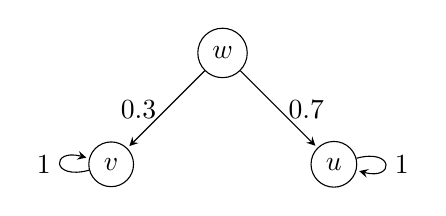
\begin{tikzpicture}[->,>=stealth,shorten >=1pt,auto,node distance=2cm]
        
        % Nodes
        \node[circle,draw] (w) {$w$};
        \node[circle,draw,below left of=w] (v) {$v$};
        \node[circle,draw,below right of=w] (u) {$u$};
        
        % Edges
        \path (w) edge node[left] {$0.3$} (v)
              (w) edge node[right] {$0.7$} (u)
              (u) edge [loop right] node {$1$} (v)
              (v) edge [loop left] node {$1$} (v);
        
        \end{tikzpicture}
        \end{minipage}\begin{minipage}{0.48\linewidth}
        \centering
            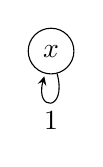
\begin{tikzpicture}[->,>=stealth,shorten >=1pt,auto,node distance=2cm]
        
        % Nodes
        \node[circle,draw] (x) {$x$};
        
        % Edges
        \path (x) edge [loop below] node {$1$} (x);
        
        \end{tikzpicture}
        \end{minipage}
    \caption{Two models whose states are bisimilar but not sabotage/bridge/swap bisimilar.}
    \label{ex_not_bis}
\end{figure}

\subsection{Invariance Theorems for Probabilistic Relation-Changing Modalities}
\label{sec:invariance}

In this section we will start by proving that the notions of bisimulation we just introduced, are adequate for the respective logic. Our first result concerns a minimal condition we aim to satisfy, namely that two probabilistic models that are bisimilar for some of the notions from previous section, satisfy the same set of formulas of the respective logic. 

\begin{theorem}[Invariance]\label{th:invariance}
    Let $\model=(W,P,V)$ and $\model'=(W',P',V')$ be two probabilistic Kripke models and let $E\subseteq \big((W\times Prob(W)\big) \times \big(W'\times Prob(W')\big)$ be a sabotage (resp. bridge/swap) bisimulation. Then, $(w,P)E(w',P')$ implies $\model,w\equiv_{\mathsf{sb}}\model',w'$ (resp. $\model,w\equiv_{\mathsf{br}}\model',w'$/$\model,w\equiv_{\mathsf{sw}}\model',w'$).
\end{theorem}

\begin{proof}
    We prove the theorem by induction over the structure of formulas. Moreover, we will prove a more general result: for all well-formed matrices ${Q}$ and ${Q'}$, $(w,{Q})E(w',{Q}')$ implies $(W,{Q},V),w\equiv_{\mathsf{sb}}(W',{Q}',V'),w'$.  
    We firstly consider the sabotage semantics.
    
    \medskip
    \noindent \underline{Base case:}
    \begin{itemize}
        \item If $\varphi\in\prop$, then the result follows from \textbf{(atom)}  from Def. \ref{switch_bis}.
    \end{itemize}
    
    \noindent \underline{Inductive cases:}
    \begin{itemize}
        \item If $\varphi=\neg\psi$, then $(W,{Q},V),w\models\neg\psi$ iff $(W,{Q},V),w\not\models\psi$. By IH, $(W',{Q}',V'),w'\not\models\psi$, and then 
        $(W',{Q}',V'),w'\models\neg\psi$.

        \item If $\varphi=\psi\vee\chi$, then $(W,{Q},V),w\models\psi\vee\chi$ iff, by definition, $(W,{Q},V),w\models\psi$ or $(W,{Q},V),w\models\chi$. Thus, by IH, we obtain that $(W',{Q}',V'),w'\models\psi$ or $(W',{Q}',V'),w'\models\chi$, hence $(W',{Q}',V'),w'\models\psi\vee\chi$.

        \item If $\varphi=\Diamond_\rho \psi$, then $(W,{Q},V),w\models \Diamond_\rho \psi$ iff $\sum_{\{v \in W \mid (W,{Q},V),v\models\psi\}} {Q}(w,v) \geq \rho$. Note that (by Def.~\ref{switch_bis}) 

        \[
            \begin{aligned}
            & \sum_{\{v\in W \mid (W,{Q},V),v\models\psi\}} {Q}(w,v) \\
            \leq & \sum_{\{v'\in W' \mid  (v',{Q}')\in \bigcup_{\{v \in W \ \mid \ (W,{Q},V),v\models\psi\}}E[(v,{Q})]\}} {Q}'(w',v') \\ 
            \leq & \sum_{\{v' \in W' \mid  (W',{Q}',V'),v'\models\psi\}} {Q}'(w',v')
            \end{aligned}    
        \]
        (since $(v,{Q})E(v',{Q}')$, and by IH). Moreover, by using the same reasoning we can conclude that
        \[
            \begin{aligned}
            \sum_{\{v \in W \mid  (W,{Q},V),v\models\neg\psi\}}{Q}(w,v) &\leq 
            \sum_{\{v' \in W' \mid (W',{Q}',V'),v'\models\neg\psi)\}} {Q}'(w',v').
            \end{aligned}
        \]
        Since for all $w\in W$, $\sum_{v \in W}{Q}(w,v)=1$ and for all $w'\in W'$,  it holds that $\sum_{v' \in W'}{Q}(w',v')=1$, we get  
        \[
            \sum_{\{v\in W \ \mid \ (W,{Q},V),v\models\psi\}}{Q}(w,v)= \sum_{\{v' \in W' \mid (W',{Q}',V'),v'\models\psi\}} {Q}'(w',v'),
        \]  
        because every $w\in W\cup W'$  satisfies either $\psi$  or $\neg\psi$. 
        Hence, we can conclude $(W,{Q},V),w\models \Diamond_\rho \psi$ iff 
        $(W',{Q}',V'),w'\models \Diamond_\rho \psi$.

        % \item If $\varphi= \blacklozenge_\rho \psi$, then $(W,{Q},V),w\models \blacklozenge_\rho \psi$ iff exists  $v\in W$ s.t.  $\rho\leq {Q}(w,v) < 1$,  and  $(W,{Q}^{-(w,v)}_\rho,V), v \models\psi$. From \textbf{(sab-zig)} in Def.~\ref{switch_bis}, there exists $v'\in W'$ s.t. ${Q}(w,v)\leq {Q}'(w',v') < 1$  and $(v,{Q}^{-(w,v)}_\rho)E(v',{Q}'^{-(w',v')}_\rho)$. Thus, by IH, exists $v'\in W'$, s.t. $\rho\leq {Q}'(w',v')<1$, and $(W',{Q}'^{-(w',v')}_\rho,V'), v' \models\psi$, and therefore $(W',{Q}',V'), w'\models\blacklozenge_\rho\psi$.
        \item Suppose $\varphi= \blacklozenge_\rho \psi$ and $(W,{Q},V),w\models \blacklozenge_\rho \psi$. Then, there exists  $v\in W$ such that  $\rho\leq {Q}(w,v) < 1$,  and  $(W,{Q}^{-(w,v)}_\rho,V), v \models\psi$. From \textbf{(sab-zig)} in Def.~\ref{switch_bis}, there exists $v'\in W'$ such that $\rho\leq {Q}'(w',v') \neq 1$  and $(v,{Q}^{-(w,v)}_\rho)E(v',{Q}'^{-(w',v')}_\rho)$. Thus, by IH, exists $v'\in W'$, s.t. $\rho\leq {Q}'(w',v')<1$, and $(W',{Q}'^{-(w',v')}_\rho,V'), v' \models\psi$, and therefore, we conclude that $(W',{Q}',V'), w'\models\blacklozenge_\rho\psi$.

        The reciprocal implication is proved analogously, using \textbf{(sab-zag)}.
    \end{itemize}

    Therefore, since $P$ and $P'$ are well-formed and they are s.t. $(w,P)E(w',P')$, we can conclude that $\model,w\equiv_{\mathsf{sb}}\model',w'$.
    
    %$\model,w\models \blacklozenge_\rho \varphi$ \ iff \ $\exists \ v\in W \mbox{ s.t. }  \ P(w,v)\geq \rho, \mbox{ and } \model^{-(w,v)}_\rho, v \models\varphi$

   % By definition of bisimulation, $\exists \ v'\in W'$ s.t. $(w',u')\in E$ and $P'(w',v')=P(w,v)$. Also, Lemma \ref{lemma} guarantees that $E$ is still a bisimulation between $\model^{-(w,v)}_\rho$ and $\model'^{-(w',v')}_\rho$. Thus, by induction hypothesis, we deduct:

    %$\exists \ v'\in W' \mbox{ s.t. }  \ P'(w',v')\geq \rho, \mbox{ and } \model^{-(w',v')}_\rho, v' \models\varphi$ iff $\model',w'\models \blacklozenge_\rho \varphi$

   % The opposite implication is proved analogously.
    The result for bridge semantics is obtained using the analogous reasoning. We prove only the case for formulas with the $\blacklozenge$ modality:

    % \begin{itemize}
    %     \item Suppose $\varphi=\blacklozenge_\rho\psi$ and $(W,{Q},V),w\models\blacklozenge_\rho\psi$. Then there is $v\in W$ such that
    %         ${Q}(w,v)+\rho\leq 1
    %         \quad\text{and}\quad
    %         (W,{Q}^{+(w,v)}_\rho,V),v\models\psi$. 
    %     By \textbf{(br-zig)} in Def.~\ref{switch_bis}, there exists $v'\in W'$ such that
    %     \[
    %         {Q}(w,v')\geq{Q}'(w',v')
    %         \quad\text{and}\quad
    %         (v,{Q}^{+(w,v)}_\rho)E(v',{Q}'^{+(w',v')}_\rho).
    %     \]
    %     Therefore,
    %     \[
    %         {Q}'(w',v')+\rho
    %         \leq{Q}(w,v')+\rho
    %         \leq 1.
    %     \]
    %     By the induction hypothesis,
    %     \[
    %         (W',{Q}'^{+(w',v')}_\rho,V'),v'\models\psi.
    %     \]
    %     Therefore,
    %     \[
    %         (W',{Q}',V'),w'\models\blacklozenge_\rho\psi.
    %     \]
    % \end{itemize}
 \begin{itemize}
        \item Suppose $\varphi=\blacklozenge_\rho\psi$ and $(W,{Q},V),w\models\blacklozenge_\rho\psi$. Then, there is $v\in W$ such that
            ${Q}(w,v)+\rho\leq 1$ and $(W,{Q}^{+(w,v)}_\rho,V),v\models\psi$. 
        By \textbf{(br-zig)} in Def.~\ref{switch_bis}, there exists $v'\in W'$ s.t. 
        ${Q}'(w',v') + \rho \leq 1$ and $(v,{Q}^{+(w,v)}_\rho)E(v',{Q}'^{+(w',v')}_\rho)$. 
        % Therefore,
        % \[
        %     {Q}'(w',v')+\rho
        %     \leq{Q}(w,v')+\rho
        %     \leq 1.
        % \]
        By IH, we get $(W',{Q}'^{+(w',v')}_\rho,V'),v'\models\psi$. 
        Therefore, we can conclude $(W',{Q}',V'),w'\models\blacklozenge_\rho\psi$. 
    \end{itemize}
    The reciprocal implication is obtained analogously by using \textbf{(br-zag)}.


    It remains the verify that the result also holds under swap semantics:
    \begin{itemize}
            \item Suppose $\varphi=\blacklozenge_\rho\psi$ and $(W,{Q},V),w\models\blacklozenge_\rho\psi$. Then, there exists $v\in W$ such that
                $\rho \leq {Q}(w,v) \neq 1$, 
                ${Q}(v,w)+\rho\leq 1$, and
                $(W,{Q}^{*(w,v)}_\rho,V),v\models\psi$. 
            By \textbf{(sw-zig)} in Def.~\ref{switch_bis}, there exists $v'\in W'$ such that
               $\rho\le Q'(w',u')\neq 1$, $Q'(u',w')+\rho\le 1$ 
                and 
                $(v,{Q}^{*(w,v)}_\rho)E(v',{Q}'^{*(w',v')}_\rho)$. 
            Thus, by IH, we obtain 
            $(W',{Q}'^{*(w',v')}_\rho,V'),v'\models\psi$. 
            Therefore, 
                $(W',{Q}',V'),w'\models\blacklozenge_\rho\psi$.
        \end{itemize}
         Once again, the reciprocal implication is obtained using \textbf{(sw-zag)}.
    % \begin{itemize}
    %     \item Suppose $\varphi=\blacklozenge_\rho\psi$ and $(W,{Q},V),w\models\blacklozenge_\rho\psi$. Then there is $v\in W$ such that
    %     \begin{itemize}
    %         \item $\rho \leq {Q}(w,v) \neq 1$, 
    %         \item ${Q}(v,w)+\rho\leq 1$, and
    %         \item $(W,{Q}^{*(w,v)}_\rho,V),v\models\psi$.
    %     \end{itemize}
    %     By \textbf{(sw-zig)} in Def.~\ref{switch_bis}, there exists $v'\in W'$ such that
    %     \begin{itemize}
    %         \item ${Q}(w,v) \leq {Q}'(w',v') < 1$, 
    %         \item ${Q}'(v',w') \leq {Q}(v,w) $, and
    %         \item $(v,{Q}^{*(w,v)}_\rho)E(v',{Q}'^{*(w',v')}_\rho)$.
    %     \end{itemize}
    %     Then,
    %     \begin{itemize}
    %         \item $\rho \leq {Q}(w,v) \leq {Q}'(w',v') < 1$, and 
    %         \item ${Q}'(v',w') + \rho \leq {Q}(v,w) + \rho \leq 1$.
    %     \end{itemize}
    %     By IH,
    %     \[
    %         (W',{Q}'^{*(w',v')}_\rho,V'),v'\models\psi.
    %     \]
    %     Therefore,
    %     \[
    %         (W',{Q}',V'),w'\models\blacklozenge_\rho\psi.
    %     \]
    % \end{itemize}
    %Here we note that the additional condition \textbf{(univ)} (i.e., for all $w\in W$,  $w'\in W'$, $E[\{(w,P)\}]\neq \emptyset \neq E^{-1}[\{(w',P')\}]$)  ensures that it is not possible to create a bridge to a new state that was not previously bisimilar to any other. This is not required for sabotage because the probability assigned to edges with probability of $0$ is never changed.
\end{proof}

%$Prob(W)$ is the set of all probabilistic matrices $W\times W$

%\textcolor{red}{The generalization of bisimulation is not straightforward}
%\begin{definition}[Bridge-bisimulation]
 %   Given a  probabilistic Kripke model  $\M=(S,P, V)$, a \emph{bisimulation} on $\M$ is an equivalence relation $B$ on $S$ such that it $s B s'$ we have
 
 %   A relation $Z\subseteq (W \times Prob(W) \times (W'\times Prob(W))$ is a \emph{bridge bisimulation} if and only if, $(w,E)Z(w',E')$ implies:
 %   \begin{description}
  %      \item[atom:] $w\in V(p)$ iff $w'\in V'(p)$, for all $p\in\prop$;
        %\item[sab-zig$_{x}$:] if there is $v\in W$ s.t. $E(w,v)\geq x$ then there is $v'\in W'$ s.t. $E'(w',v')\geq x$ and $(v,\modsabx{E}{(w,v)})Z(v,\modsabx{E'}{(w',v')})$ ;
   %     \item[bridge-zig:] for any $v\in W$ such that $E(w,v)< x$, exists $v'\in W'$ s.t.  $x > E'(w',v')$ and $(v,\modbridx{E}{(w,v)})Z(v',\modbridx{E'}{(w',v')})$;
        % \item[zig:] for any $v\in W$  there is $v'\in W'$ s.t. $E'(w',v')\geq E(w,v)$ and $vZv'$% and $(v,\modsabx{E}{(w,v)})Z(v,\modsabx{E'}{(w',v')})$;
        %\item[sab-zag$_{x}$:] if there is $v'\in W'$ s.t. $E'(w',v')\geq x$ then there is $v\in W$ s.t. $E(w,v)\geq x$ and $(v,\modsabx{E}{(w,v)})Z(v,\modsabx{E'}{(w',v')})$.
    %    \item[bridge-zag:] for any $v'\in W'$ such that $E'(w',v')< x$, exists $v\in W$ s.t.  $x > E(w,v)$ and $(v,\modbridx{E}{(w,v)})Z(v',\modbridx{E'}{(w',v')})$.
    %\end{description}
    %We say that $\model,w$ and $\model',w'$ are $x$-bridge bisimilar (denoted $\model,w\bridbisim_x\model',w'$) iff there is a bridge bisimulation $Z$ such that $(w,R)E(w',R')$. They are bridge bisimilar (denoted $\model,w\bridbisim\model',w'$), if they are $x$-bridge bisimilar for all $x{\in}[0,1]$.
%\end{definition}


%\begin{theorem}[Invariance under bridge-bisimulation]\label{th:invariance-bridge}
 %   Let $\model=(W,R,V)$ and $\model'=(W',R',V')$ be two fuzzy Kripke models. If $\model,w\bridbisim\model',w'$, then  $\truthset{\varphi}{\model}{w} = \truthset{\varphi}{\model'}{w'}$, for every formula $\varphi\in\form_{br}$.
%\end{theorem}

We conclude this section with an example of relation-changing bisimulation and the use of our invariance theorems. 

\begin{example}
Let $\prop=\{p\}$ and consider the two probabilistic Kripke models, as shown in Fig. \ref{ex_r-bis}. We denote the model on the left by $\model=(W,P,V)$ and the one on the right by $\model'=(W',P',V')$, with $V(p)=\{u,v,x\}$ and $V'(p)=\{u',v',x',y'\}$.

\begin{figure}[!ht]
        \begin{minipage}{0.48\linewidth}
        \centering
            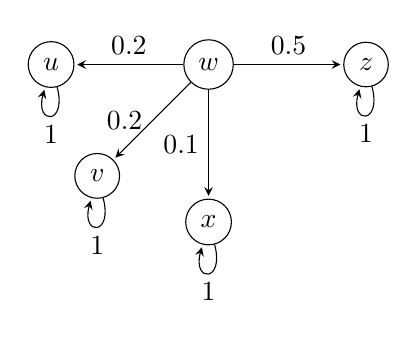
\begin{tikzpicture}[->,>=stealth,shorten >=1pt,auto,node distance=2cm]
        
        % Nodes
        \node[circle,draw] (w) {$w$};
        \node[circle,draw,below left of=w] (v) {$v$};
        \node[circle,draw,left of=w] (u) {$u$};
        \node[circle,draw,below of=w] (x) {$x$};
        \node[circle,draw,right of=w] (z) {$z$};
        
        % Edges
        \path (w) edge node[left] {$0.2$} (v)
              (w) edge node[above] {$0.2$} (u)
              (w) edge node[left] {$0.1$} (x)
              (w) edge node[above] {$0.5$} (z)
              (u) edge [loop below] node {$1$} (v)
              (v) edge [loop below] node {$1$} (v)
              (x) edge [loop below] node {$1$} (x)
              (z) edge [loop below] node {$1$} (z);
        
        \end{tikzpicture}
        \end{minipage}\begin{minipage}{0.48\linewidth}
        \centering
            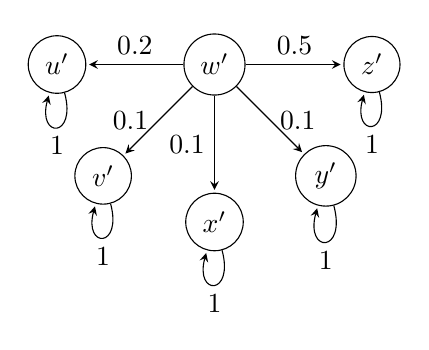
\begin{tikzpicture}[->,>=stealth,shorten >=1pt,auto,node distance=2cm]
        % Nodes
        \node[circle,draw] (w) {$w'$};
        \node[circle,draw, below left of=w] (v) {$v'$};
        \node[circle,draw, left of =w] (u) {$u'$};
        \node[circle,draw,below of=w] (x) {$x'$};
        \node[circle,draw,below right of=w] (y) {$y'$};
        \node[circle,draw,right of=w] (z) {$z'$};
        
        % Edges
        \path (w) edge node[above] {$0.2$} (u)
              (w) edge node[left] {$0.1$} (v)
              (w) edge node[left] {$0.1$} (x)
              (w) edge node[right] {$0.1$} (y)
              (w) edge node[above] {$0.5$} (z)
              (u) edge [loop below] node {$1$} ()
              (v) edge [loop below] node {$1$} (v)
              (x) edge [loop below] node {$1$} (x)
              (y) edge [loop below] node {$1$} (y)
              (z) edge [loop below] node {$1$} (z);
        \end{tikzpicture}
        \end{minipage}
    \caption{Example of models with sabotage bisimilar states.}
    \label{ex_r-bis}
\end{figure}

It is possible to verify that the following relation is a sabotage-bisimulation:
    \[
    \begin{array}{l@{\,}l}
        E = & \{\big((w,P),(w',P')\big),$ $\big((z,P),(z',P')\big)\} \\ 
            & \cup \ \{(t,P)\times (t',P'): \ t\in\{u,v,x\}\text{ and }t'\in\{u',v',x',y'\}\}\\
            & \cup \ \{(z,P^{-(w,z)}_\rho)\times (z',P'^{-(w',z')}_\rho): \ \rho\in ]0,0.5]\}\\
            &\cup \ \{(t,P^{-(w,t)}_\rho)\times (u',P'^{-(w',u')}_\rho): \ t\in\{u,v\}\text{ and }\rho\in]0,0.2]\}\\
            & \cup \ \{(x,P^{-(w,x)}_\rho)\times (t',P'): \ t'\in\{v',x',y'\}\text{ and }\rho\in]0,0.1]\}
    \end{array}
    \]
Therefore, $w$ is bisimilar to $w'$, $z$ is bisimilar to $z'$ and $u$, $v$, $x$ are bisimilar to $u'$, $v'$, $x'$, $y'$. Furthermore, the two models above satisfy the same sabotage formulas by Theorem~\ref{th:invariance}.

\end{example}

\subsection{Hennessy-Milner Results}
\label{sec:henmilner}

In this section, we will devote ourselves to the proof of Hennessy-Milner results~\cite{vanbenthem1977modal}. Concretely, we will show that under certain circumstances, the converse of Theorem~\ref{th:invariance} holds. As it is usual in modal logics, these conditions involve some finiteness constraint, namely image finiteness or finite models. Below we define classes of models satisfying those conditions, called in general \emph{Hennessy-Milner classes} (see, e.g.,~\cite{BlackburnRV01}).


\begin{definition}
    \label{def:image-finite}
A model $\model=(W,P,V)$ is \emph{image finite} if for all $w\in W$, we have that the set $\{v \in W \mid P(w,v)>0\}$ is finite. We say that $\model$ is \emph{finite} if its set of states $W$ is finite.
\end{definition}
%
\begin{remark}\label{rem:well-formed}
   Let $\model=(W,P,V)$ be an image finite probabilistic Kripke model.  Then, for all ${Q}$ that is well-formed from $P$ for sabotage, we have that $\model=(W,{Q},V)$ is also image finite.
\end{remark}

The two types of models will be relevant in our case. Such as it is done for non-probabilistic sabotage in~\cite{ArecesFH15}, image finite suffices to obtain a Hennessy-Milner class. However, this is not the case for bridge, as in infinite model, there exist  infinitely many possible new edges that can be added. In our probabilistic setting, this situation naturally persists.


\begin{theorem}
    [Hennessy-Milner for sabotage]
     Let $\model=(W,P,V)$ and $\model'=(W',P',V')$ be two image finite probabilistic Kripke models. Let ${Q},{Q'}$ be two well-formed probabilistic matrices for sabotage w.r.t. $P,P'$ respectively.  
    Then, $(W,{Q},V),w\equiv_{\mathsf{sb}}(W',{Q}',V'),w'$ implies there exists a sabotage bisimulation $E$ such that $(w,{Q})E(w',{Q}')$.
\end{theorem}
\begin{proof}
We will prove the relation given by:
% \textcolor{blue}{RF: $\bar P$ and ${Q'}$ must all be image finite, to make sure that we always work with image finite models}
\begin{align*}
    E := & \{ ((u,{Q}),(u',{Q}')) \mid  (W,{Q},V), u \equiv_{\mathsf{sb}} (W',{Q}',V') , u' \text{ and } \\
    & \text{ ${Q},{Q'}$ are well-formed for sabotage from $P,P'$ respectively} \} 
\end{align*}
is a sabotage bisimulation. Thus, for every $\big((w,{Q}) ,(w',{Q}')\big)\in E$, we have to prove that conditions \textbf{(atom)}, \textbf{(sab-zig)}, \textbf{(sab-zag)}, and \textbf{(p-zigzag)} hold. Notice that by Remark~\ref{rem:well-formed}, models whose underlying probability matrices are ${Q}$ and ${Q}'$, are image-finite models.
% While doing so, we will denote $\bar{\model}=(W,{Q},V)$ and $\bar{\model}'=(W',{Q}',V)$.

\begin{description}
    \item[(atom):] follows immediately from definition of $E$. 

    \item[\textbf{(sab-zig)}:] let $u \in W$ be such that $\rho \leq {Q}(w,u) \neq 1$. We have to prove that there exists $u'$ such that items 1 and 2 from \textbf{(sab-zig)} hold. First, notice that, since $\rho \neq 1 $, we have that $(W,{Q},V), w \models \blacklozenge_{\rho} \top$. Thus, we also have that $(W',{Q}',V'), w' \models \blacklozenge_{\rho} \top$ (by definition of $E$). Therefore, there exists $u' \in W'$ such that $\rho \leq {Q}'(w',u') \neq 1$, proving item 1. To prove item~2, aiming for a contradiction we assume that for every $u' \in W'$ such that $ \rho \leq {Q}'(w', u') < 1$,  we have $\big(\big(u, {Q}_{\rho}^{-(w,u)}\big), \big(u', {Q}'^{-(w',u')}_{\rho}\big)\big) \notin E$. So, for each such $u'$ there exists $\varphi'$ such that $(W,{Q}^{-(w,u)}_{\rho},V),u\models \varphi'$ and $(W',{Q}'^{-(w',u')}_{\rho},V'),u'\not\models \varphi'$. Since $(W',{Q}'^{-(w',u')}_{\rho},V')$ is image finite, we have only a finite set $\{u'_1,\dots,u'_n\}$ of worlds satisfying the condition. Thus there are $\{ \varphi_1,\dots,\varphi_n \}$ such that $(W,{Q}^{-(w,u)}_{\rho},V),u\models \varphi_i$ and $(W',\bar{P'_{\rho}}^{-(w',u'_i)},V'),u'_i\not\models \varphi_i$. Let us define $\varphi = \bigwedge \varphi_i$, we get a contradiction because $(W,{Q},V), w \models \blacklozenge_{\rho} \varphi$ but $(W',{Q}',V'), w' \not\models \blacklozenge_{\rho} \varphi$. Hence, item 2 holds. Condition \textbf{(sab-zag)} follows in an analogous way.

    \item[\textbf{(p-zigzag)}:] 
    let $U \subseteq W$ and set $\rho = \sum_{u \in U} {Q}(w,u)$. We define the following subsets of $W'$:
    \begin{align*}
          U' &= \{ u' \in W'\mid \text{there exists } u\in U \text{ such that } (u',{Q}')\in E[(u,{Q})] \} \\
          T' &= W' \setminus U' 
    \end{align*}
    Also we define $U_0 = \{u\in U \mid {Q}(w,u) > 0 \}$ and $T'_0 = \{u'\in T' \mid {Q}'(w',u') > 0\}$. Since the models are image finite, $U_0$ and $T'_0$ are finite. Take $u\in U_0$ and $v' \in T'_0$. Since $(v', {Q}') \notin E[(u,{Q})]$, there is $\varphi_{v'}^{u}\in\form $ such that $(W,{Q},V) , u \models \varphi_{v'}^{u}$ and $(W',{Q}',V') , v' \not\models \varphi_{v'}^{u}$. Clearly, the formula
    \[
        \varphi = \bigvee_{u\in U_0} \bigwedge_{v'\in T'_0} \varphi_{v'}^{u}
    \]
    is well-formed, by finiteness of $U_0$ and $T'_0$. 
    By construction, $(W,{Q},V), w \models \Diamond_\rho \varphi$, so $(W',{Q}',V') , w' \models \Diamond_\rho \varphi$ necessarily holds. Thus,
    \[
        \sum_{\{u'\in W' \mid (W',{Q}',V'),u' \models \varphi \}}{Q}(w',u')\geq \rho.
    \]
    Finally, observe that 
    \[ 
        \begin{array}{lcl}            
            W'\setminus T'_0 & =& \{u'\in W' \mid  (u',{Q}')\notin E[(u,{Q})] \text{ or } {Q}'(w',u')=0\} \\
                            & =&  U' \cup (T'\setminus T'_0)
        \end{array}
    \]
    From that observation, we obtain $\{u' \in W' \mid (W',{Q}',V'),u' \models \varphi \} \subseteq W' \setminus T'_0 = U' \cup (T' \setminus T'_0) $, yielding the following inequalities:
    \begin{align*}
        \rho &\leq \sum_{\{u'\in W' \mid (W',{Q}',V'),u' \models \varphi \}}{Q}(w',u') \\
        &\leq \sum_{u'\in U'\cup (T'\setminus T'_0)}{Q}(w',u')\\
        &= \sum_{u'\in U'}{Q}(w',u') + \sum_{T'\setminus T'_0}{Q}(w',u')\\
        &= \sum_{u'\in U'}{Q}(w',u') + 0 \qedhere
    \end{align*}
    %let $U \subseteq W$ and set $\rho = \sum_{u \in U} P(w,u)$. We define the following two subsets of $W'$:
    %    \begin{align*}
      %      U' &= \{ u' \mid \text{there exists } u\in U \text{ such that } (u',P')\in E[(u,P)] \} \\
      %     V' &= W' \setminus U' 
     %   \end{align*}
    %We want to show that $\sum_{u'\in U'} P'(w',u') \geq \rho$. Given $u\in U$ and $v' \in V'$, since $(v', P') \notin E[(u,P)]$, there is $\varphi_{v'}^{u}\in\form $ such that $\model , u \models \varphi_{v'}^{u}$ and $\model' , v' \not\models \varphi_{v'}^{u}$. As the models are image finite, we have that $\varphi = \bigvee_{u\in U} \bigwedge_{v'\in V'} \varphi_{v'}^{u} $ belongs to $\form$.
    %By construction, it follows that $\model , w \models \Diamond_\rho \varphi$, so $\model' , w' \models \Diamond_\rho \varphi$ and since $\varphi$ only holds for $U'$, we have that $\sum_{u'\in U'}P(w',u')\geq \rho $.
\end{description}
\end{proof}

Once a Hennessy-Milner result for sabotage has been established over models with image finite, we proceed to prove a similar result for bridge. Similarly to its non probabilistic counterpart, for bridge the result holds over finite models.

\begin{theorem}
    [Hennessy-Milner for bridge]
     Let $\model=(W,P,V)$ and $\model'=(W',P',V')$ be two finite probabilistic Kripke models.
    Let ${Q},{Q'}$ be two well-formed probabilistic matrices for bridge w.r.t. $P,P'$ resp.  
    Then, $(W,{Q},V),w\equiv_{\mathsf{br}}(W',{Q}',V'),w'$ implies there exists a bridge bisimulation $E$ s.t. $(w,{Q})E(w',{Q}')$.
\end{theorem}
\begin{proof}
% Let us define $E$ like in the sabotage case but using the $\equiv_{\mathsf{br}}$ notion. 
We will prove the relation given by:
\begin{align*}
    E := & \{ ((u,{Q}),(u',{Q}')) \mid  (W,{Q},V), u \equiv_{\mathsf{br}} (W,{Q}',V) , u ' \text{ and} \\
    & \text{ ${Q},{Q'}$ are well-formed for bridge from $P,P'$ respectively} \} 
\end{align*}
is a bridge bisimulation. Again, every well-formed ${Q},{Q'}$ are guaranteed to be finite provided that $\model$ and $\model'$ are finite models.

We need to prove that, for  $\big((w,{Q}) ,(w',{Q}')\big)\in E$, conditions \textbf{(atom)}, \textbf{(br-zig)}, \textbf{(br-zag)}, and \textbf{(p-zigzag)} hold. 

\begin{description}
    \item[(atom):] follows immediately from definition of $E$. 

    % \item[(univ):] \textcolor{blue}{To be completed?}

    \item[\textbf{(br-zig)}:] let $u \in W$ be such that ${Q}(w,u) + \rho \leq 1 $. We have to prove that there exists $u'$ such that items 1 and 2 from \textbf{(br-zig)} hold. As in the case for sabotage, it holds that $(W,{Q},V) , w \models \blacklozenge_{\rho} \top $. Since $(w,{Q})E(w',{Q}')$, we have that $(W',{Q}',V') , w' \models \blacklozenge_{\rho} \top $, so there exists $u'$ such that ${Q}'(w',u') + \rho \leq 1$. Thus, item 1 holds. Now, aiming for a contradiction, let us assume item 2 does not hold, i.e., for every $u'\in W'$ such that ${Q}'(w',u') + \rho \leq 1$, we have that $\big ( \big ( u, {Q}_{\rho}^{+(w,u)} \big ), \big ( u',{Q}'^{+(w',u')}_{\rho}\big )\big ) \notin E$. Therefore, for each $u'$ such that ${Q}'(w',u') + \rho \leq 1 $, there exists $\varphi_{u'}$ that satisfies that $(W,{Q},V) , u \models \varphi_u'$ and $(W',{Q}',V') , u' \not \models \varphi_u'$. Since $W'$ is finite, we can define $\varphi = \blacklozenge_\rho \bigwedge \varphi_{u'}$. This yields a contradiction, since $(W,{Q},V) , w \models \varphi$ and $(W',{Q}',V') , w' \not \models \varphi$, hence proving item 2. Condition \textbf{(br-zag)} follows in an analogous way.
    %     \begin{align*}
    %         {Q}'(w',u') + \rho &< 1 \\
    %         {Q}'(w',u') + 1 - {Q}(w,u) - \delta &< 1 \\
    %         {Q}'(w',u') &< {Q}(w,u) + \delta  
    %     \end{align*}
    % Since it holds for every $\delta > 0$, we can take the limit as $\delta$ approaches zero, and we get ${Q}'(w',u') \leq  {Q}(w,u)$. 
    
    \item[\textbf{(p-zigzag)}:] For $U \subseteq W$, let $\rho = \sum_{u \in U} {Q}(w,u)$. Define the following sets:
        \begin{align*}
            U' &= \{ u' \in W' \mid \text{there exists } u\in U \text{ such that } (u',{Q}')\in E[(u,{Q})] \} \\
            T' &= W' \setminus U' 
        \end{align*}
    We need to show that $\sum_{u'\in U'} {Q}'(w',u') \geq \rho$. Given $u\in U$ and $v'~\in~T'$, since $(v', {Q}') \notin E[(u,{Q})]$, there is $\varphi_{v'}^{u}\in\form $ such that $(W,{Q},V) , u \models \varphi_{v'}^{u}$ and $(W',{Q}',V') , v' \not\models \varphi_{v'}^{u}$. As the models are finite, we have that $\varphi = \bigvee_{u\in U} \bigwedge_{v'\in V'} \varphi_{v'}^{u} $ belongs to $\form$.
    By construction, $(W,{Q},V) , w \models \Diamond_\rho \varphi$, so $(W'{Q}',V') , w' \models \Diamond_\rho \varphi$. Since $\varphi$ only holds for $U'$, we have that
    \[
        \sum_{u'\in U'}{Q}(w',u')\geq \rho. \qedhere
    \]
\end{description}
\end{proof}


We finish this section with the corresponding Hennessy-Milner result under swap semantics. 

\begin{theorem}
    [Hennessy-Milner for swap]
    Let $\model=(W,P,V)$ and $\model'=(W',P',V')$ be two image finite probabilistic Kripke models. Let ${Q},{Q'}$ be two well-formed probabilistic matrices for swap w.r.t. $P,P'$ respectively.  
    Then, $(W,{Q},V),w\equiv_{\mathsf{sw}}(W',{Q}',V'),w'$ implies there exists a swap bisimulation $E$ such that $(w,{Q})E(w',{Q}')$.
\end{theorem}
\begin{proof}
We will prove the relation given by:
\begin{align*}
    E := & \{ ((u,{Q}),(u',{Q}')) \mid  (W,{Q},V), u \equiv_{\mathsf{sw}} (W,{Q}',V) , u ' \text{ and} \\
    & \text{ ${Q},{Q'}$ are well-formed for swap from $P,P'$ respectively} \} 
\end{align*}
is a swap bisimulation. % Again, every well-formed ${Q},{Q'}$ are guaranteed to be finite provided that $\model$ and $\model'$ are finite models.

We need to prove that, for  $\big((w,{Q}) ,(w',{Q}')\big)\in E$, conditions \textbf{(atom)}, \textbf{(sw-zig)}, \textbf{(sw-zag)}, and \textbf{(p-zigzag)} hold. 

\begin{description}
    \item[(atom):] follows immediately from definition of $E$. 

    \item[(sw-zig):] let $u \in W$ be such that $\rho \leq Q(w,u) \neq 1 $ and $Q(u,w) + \rho \leq 1$. We have to prove that there exist $u'$ such that items 1 and 2 from \textbf{(sw-zig)} hold. We can say that $(W,{Q},V) , w \models \blacklozenge_{\rho} \top $. Since $\big((w,{Q}) ,(w',{Q}')\big)\in E$, we have that $(W',{Q}',V') , w' \models \blacklozenge_{\rho} \top $, so there exists $u'$ such that $\rho \leq Q(w',u') \neq 1 $ and $Q(u',w') + \rho \leq 1$, proving item 1. To prove item 2, we assume that for every $u' \in W'$, such that $\rho \leq Q(w',u') \neq 1$ and $Q(u',w') + \rho \leq 1$, we have $\big ( \big ( u, {Q}_{\rho}^{*(w,u)} \big ), \big ( u',{Q}'^{*(w',u')}_{\rho}\big )\big ) \notin E$. So, for each $u'$ there exists $\varphi'$ such that $(W,{Q}^{*(w,u)}_{\rho},V) , u \models \varphi'$ and $(W',{Q}'^{*(w',u')}_{\rho},V') , u' \not \models \varphi'$.

\end{description}

\end{proof}